\documentclass[11pt]{article}

\usepackage[margin=1in]{geometry}
\usepackage{amsmath, amssymb, mathtools}
\usepackage{graphicx}
\usepackage{booktabs}
\usepackage{hyperref}
\usepackage{float}

\hypersetup{colorlinks=true, linkcolor=blue, citecolor=blue, urlcolor=blue}

\newcommand{\R}{\mathbb{R}}
\newcommand{\E}{\mathbb{E}}
\newcommand{\N}{\mathcal{N}}
\newcommand{\given}{\,|\,}

\title{Belief propagation for diffusion scores on Markov chains:\\
\large exact Gaussian baseline and the cost of Gaussian message closure\\
\normalsize --- summary of results ---}
\author{Giovanni Mantovani}
\date{\today}

\begin{document}
\maketitle

\section{Setting and exact identities}

The clean signal is a Markov chain $a_{1:n}$, observed through coordinatewise
Ornstein--Uhlenbeck noising at diffusion time $t>0$:
\[
  x_i = \alpha_t a_i + \sqrt{\Delta_t}\, z_i,
  \qquad
  \alpha_t = e^{-t},
  \qquad
  \Delta_t = 1 - e^{-2t},
  \qquad z_i \sim \N(0,1) \text{ i.i.d.}
\]
Two structural facts organize everything:
\begin{enumerate}
  \item \textbf{The posterior is a chain.} A Markov prior plus coordinatewise noise
  gives a posterior $p_t(a_{1:n}\given x_{1:n})$ whose factor graph is a chain, hence a
  tree, hence sum-product BP computes the posterior marginals \emph{exactly}.
  \item \textbf{The denoiser gives the score.} For every Markov prior,
  \[
    \boxed{\;
    s_i(x,t) = \partial_{x_i} \log p_t(x)
             = -\frac{x_i - \alpha_t\, m_i(x,t)}{\Delta_t},
    \qquad
    m_i(x,t) = \E[a_i \given x_{1:n}].
    \;}
  \]
\end{enumerate}
So exactness of BP is never the issue on a chain. The issue is
\emph{representation}: for a continuous non-Gaussian chain, each BP message is a whole
function of a continuous variable. Only in special cases (Gaussian: two scalars;
finite alphabet: a finite vector) do the messages close in a finite-dimensional family.

\section{Part I: the Gaussian AR(1) baseline is fully solvable}

For the stationary Gaussian AR(1) prior ($\Sigma_0(i,j)=\rho^{|i-j|}$), BP messages stay
Gaussian, and the score is also available directly by linear algebra,
$s(x,t) = -\Sigma_t^{-1}x$ with $\Sigma_t = \alpha_t^2 \Sigma_0 + \Delta_t I$.
Running both routes ($n=40$, $\rho=0.7$, $t=0.8$):
\[
  \max_i \left| s^{\mathrm{BP}}_i - s^{\mathrm{matrix}}_i \right|
  \;\approx\; 6.7\times 10^{-16},
\]
i.e.\ agreement at machine precision, matching the algebraic proof of equivalence.
This case serves as the exactly-solvable control for everything below.

\section{Part II: general chains and the two algorithms}

For non-Gaussian chains we compare two implementations of the same BP equations:
\begin{itemize}
  \item \textbf{Reference grid BP.} Messages represented on a grid of $M$ points,
  integrals by trapezoidal quadrature. Converged in $M$, this is numerically exact.
  \item \textbf{Gaussian projected BP} (assumed-density filtering style). After each exact
  message update, the outgoing message is replaced by the Gaussian with the same first two
  moments. This isolates precisely the error caused by \emph{Gaussian message closure} ---
  the approximation implicitly made when one treats a non-Gaussian problem with
  Gaussian/AMP-style machinery.
\end{itemize}
Test model: AR(1) chain with \textbf{Laplace innovations} (same correlation structure as
the Gaussian case, $\rho=0.85$, unit marginal variance, $n=50$, heavier tails).

\subsection*{Is the reference trustworthy?}

Two independent checks from the heavy runs:
\begin{itemize}
  \item \emph{Gaussian control:} grid BP vs the exact matrix score, 48 trials per $t$,
  grid sizes $M \in \{101,201,401\}$: relative score error
  $\sim 10^{-16}$--$10^{-14}$ for all diffusion times.
  \item \emph{Laplace grid convergence:} $M=401$ vs $M=801$, 16 trials per $t$: relative
  score difference $\le 6\times 10^{-6}$ at all times --- three to five orders of
  magnitude below the closure error being measured.
\end{itemize}

\section{Main result: the price of Gaussian message closure}

Figure~\ref{fig:quantiles} shows the per-trial distribution (100 trials per diffusion
time) of the relative score error
$\|s^{\mathrm{Gauss}} - s^{\mathrm{grid}}\|_2 / \|s^{\mathrm{grid}}\|_2$
of Gaussian projected BP on the Laplace chain.

\begin{figure}[H]
  \centering
  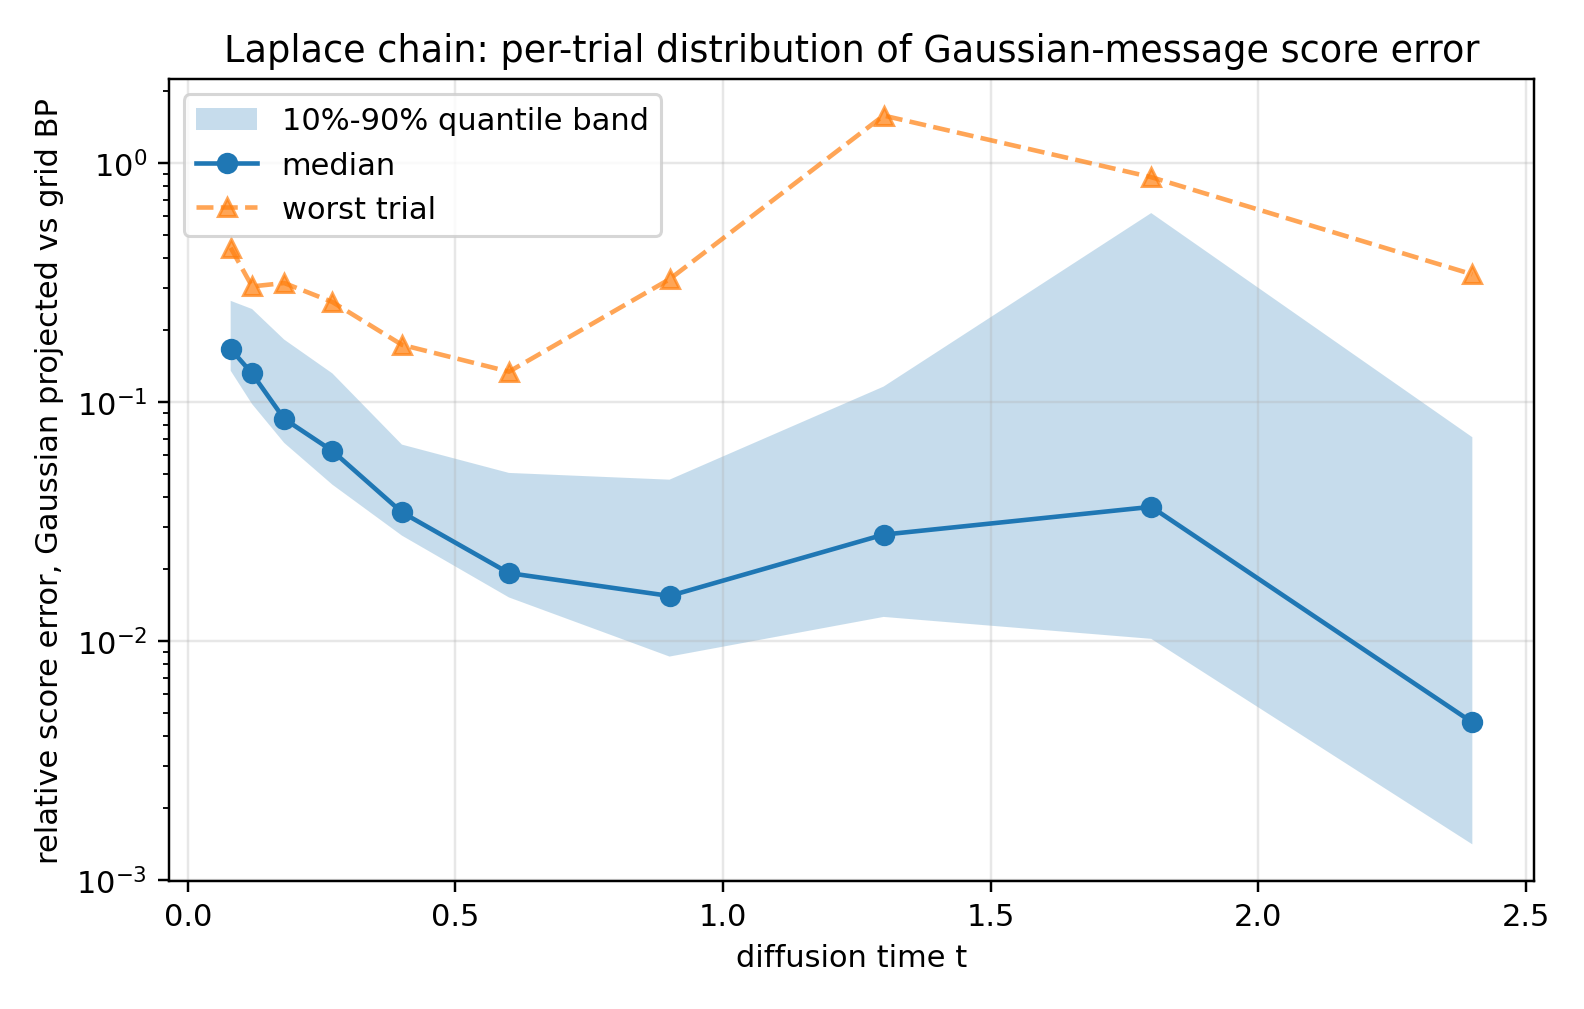
\includegraphics[width=0.86\textwidth]{../markov_gaussian_approx/outputs_heavy/per_trial/laplace_score_error_quantiles.png}
  \caption{Per-trial distribution of the Gaussian-closure score error on the Laplace
  chain ($\rho=0.85$, $n=50$, reference grid $M=401$). Small $t$: large, systematic
  error. Intermediate $t$: sub-percent. Large $t$ ($t \gtrsim 1.3$): the widening band is
  dominated by a numerical instability of moment matching, see Section~\ref{sec:instability}.}
  \label{fig:quantiles}
\end{figure}

\begin{table}[H]
\centering
\begin{tabular}{rccc}
\toprule
$t$ & closure error (wide grid) & numerical floor$^{\dagger}$ & median (100 trials) \\
\midrule
0.08 & 0.211 & $10^{-15}$ & 0.167 \\
0.18 & 0.094 & $10^{-15}$ & 0.085 \\
0.40 & 0.044 & $2\times10^{-7}$ & 0.035 \\
0.60 & 0.023 & $2\times10^{-6}$ & 0.019 \\
0.90 & 0.010 & $3\times10^{-4}$ & 0.015 \\
1.30 & 0.010 & $7\times10^{-3}$ & 0.028 \\
1.80 & --- & $0.16$ (unreliable) & --- \\
\bottomrule
\end{tabular}
\caption{Relative score error of Gaussian projected BP on the Laplace chain.
``Wide grid'' = mean over 16 trials on $[-12,12]$. $^{\dagger}$The floor is the same
algorithm run on the \emph{Gaussian} chain, where projection is exact in principle, so any
deviation is purely numerical. At $t\ge 1.8$ the floor exceeds the signal: those
entries measure implementation fragility, not closure error.}
\label{tab:closure}
\end{table}

Three regimes:
\begin{enumerate}
  \item \textbf{Small $t$ (near the data): the closure error is large and systematic.}
  At $t=0.08$ the median relative score error is $\approx 17\%$ and \emph{every one of
  100 trials} exceeds $10\%$. This is not an outlier effect. The mechanism is the exact
  identity $s^{\mathrm{Gauss}}-s^{\mathrm{grid}} = (\alpha_t/\Delta_t)\,
  (m^{\mathrm{grid}}-m^{\mathrm{Gauss}})$ (verified to $10^{-14}$ in the runs): as
  $t\to 0$ the denoiser error is amplified by $\alpha_t/\Delta_t \sim 1/(2t)$, exactly
  where the posterior is most sensitive to the non-Gaussian innovation tails.
  The \emph{direction} of the score survives better: cosine similarity $\ge 0.98$.
  \item \textbf{Intermediate $t$: Gaussianization.} By $t \approx 0.9$--$1.3$ the closure
  error drops below $1\%$: the noisy marginal has effectively Gaussianized and Gaussian
  messages are adequate.
  \item \textbf{Large $t$: an instability of naive moment matching (not closure error).}
\end{enumerate}

\section{The weak-information instability}
\label{sec:instability}

The Gaussian control run exposes an important numerical phenomenon. For
$t \gtrsim 1.8$ the likelihood precision $\alpha_t^2/\Delta_t \to 0$ and BP messages
become nearly flat. Computing first and second moments of a nearly flat function on a
finite grid is ill-conditioned, and the Gaussian projected algorithm develops rare but
catastrophic failures --- \emph{even in the purely Gaussian model}, where projection
should be exact ($0.16$ relative error at $t=1.8$; widening the grid from $[-8,8]$ to
$[-12,12]$ moves but does not remove the effect). On the Laplace chain at $t=1.8$,
$30\%$ of trials exceed $10\%$ score error for the same reason. Figure~\ref{fig:worst}
shows the worst observed failure: the projected belief detaches completely from the true
posterior mode.

\begin{figure}[H]
  \centering
  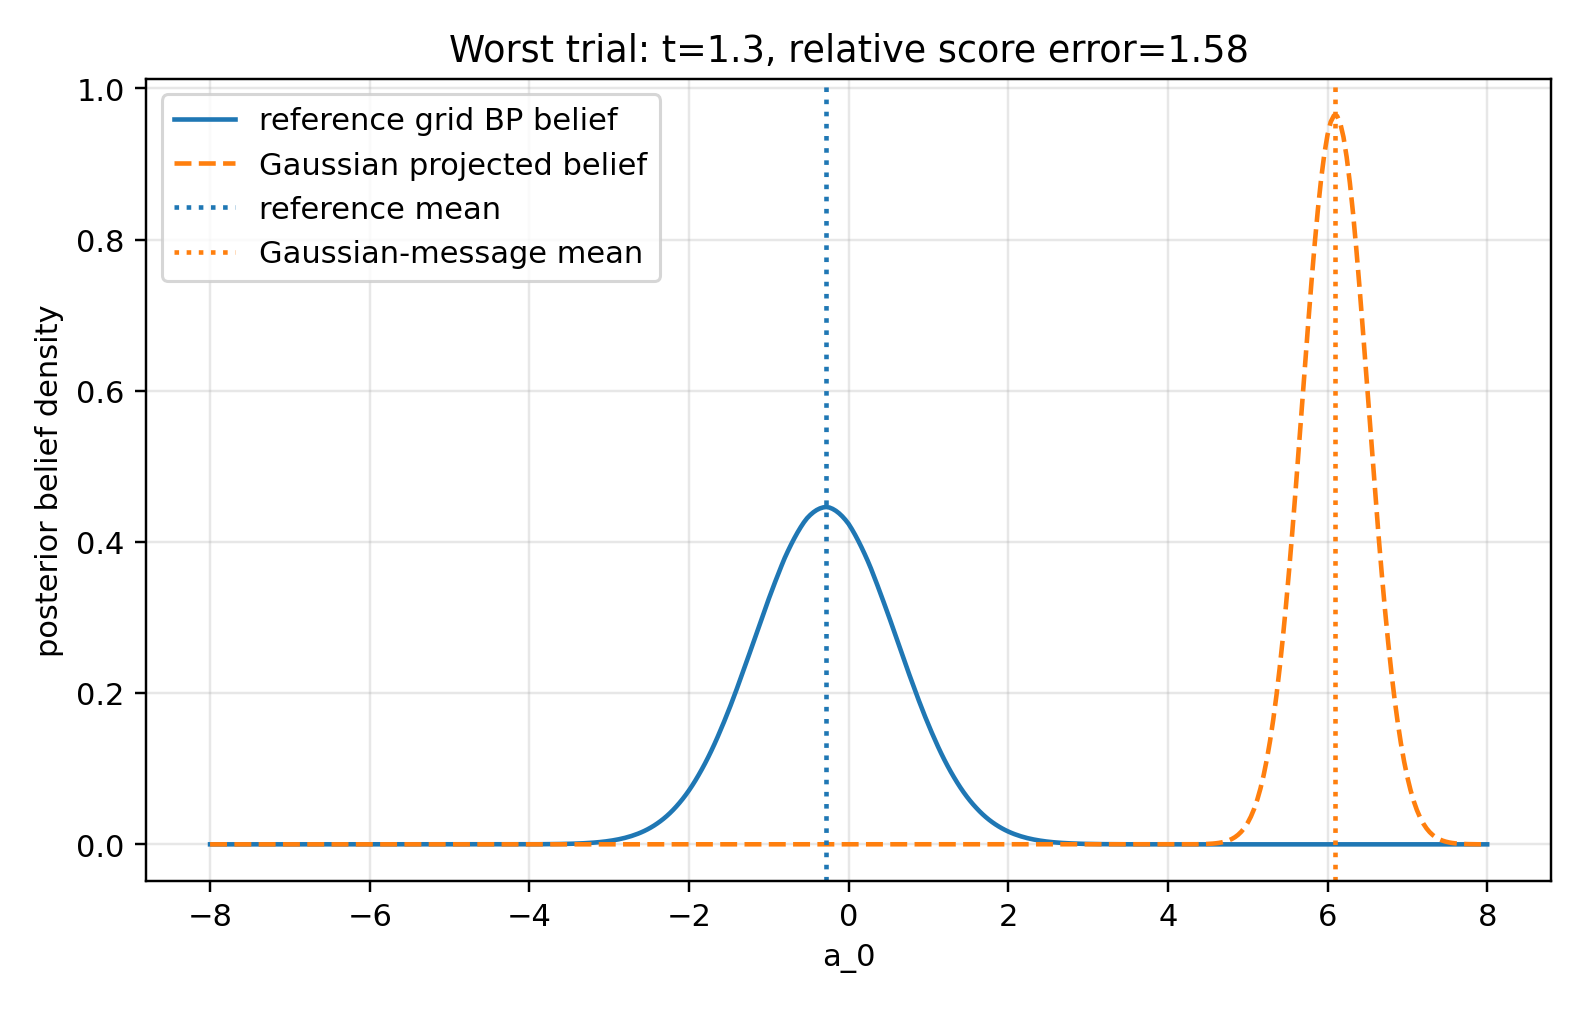
\includegraphics[width=0.82\textwidth]{../markov_gaussian_approx/outputs_heavy/per_trial/worst_case_belief.png}
  \caption{Worst failure over 1000 runs ($t=1.3$): the moment-matched message chain
  places the belief at $a_0 \approx 6.1$ while the true posterior sits at $-0.29$. A
  message-passing analogue of losing the mode.}
  \label{fig:worst}
\end{figure}

The practical lesson: message \emph{parametrization matters}. Moment matching on grids is
fragile exactly in the weak-signal regime, whereas information-form (natural-parameter)
updates --- the ones used in Gaussian BP and in AMP derivations --- handle flat messages
gracefully ($\lambda \to 0$ is a perfectly regular point). This is an argument, from a
purely numerical direction, for AMP-style parametrizations.

\section{Proposed next steps}

\begin{enumerate}
  \item \textbf{Sharper small-$t$ theory.} The measured closure error follows a clean
  monotone law in $t$. It should be possible to characterize the leading-order error in
  terms of the excess kurtosis of the innovations and the amplification factor
  $\alpha_t/\Delta_t$, and compare with the empirical curve.
  \item \textbf{Beyond two moments.} Project messages onto richer families
  (Gaussian mixtures, or an Expectation-Propagation variant with damping in natural
  parameters) and measure how quickly the small-$t$ gap closes as the family grows.
  \item \textbf{Priors with real structure.} Replace Laplace innovations with sparse
  (spike-and-slab) or bimodal innovations, where the posterior genuinely multimodalizes
  and the speciation-like regime appears at finite $t$; measure whether the closure error
  then develops a peak at intermediate $t$ rather than decaying monotonically.
  \item \textbf{Contact with AMP.} On dense graphs the same Gaussian-closure step is what
  turns BP into AMP. The chain setting gives a controlled laboratory where the exact
  answer is computable; the analogous comparison on dense/loopy models would quantify how
  much of AMP's error is Gaussian closure versus loop effects.
\end{enumerate}

\begin{thebibliography}{9}
\bibitem{BiroliMezard2023}
G. Biroli and M. M\'ezard.
\newblock Generative diffusion in very large dimensions.
\newblock arXiv:2306.03518, 2023.

\bibitem{MezardMontanari2008}
M. M\'ezard and A. Montanari.
\newblock Information, Physics, and Computation.
\newblock Oxford University Press, 2009.

\bibitem{GenovesePiana2026}
G. Genovese and A. Piana.
\newblock Derivation of the AMP equations from belief propagation for the $\ell_2$ minimisation problem.
\newblock arXiv:2602.15191, 2026.
\end{thebibliography}

\end{document}
